\section{Einführung}
	\begin{frame}
		\frametitle{Einführung: Linear seperierbare Daten}
			\begin{figure}
					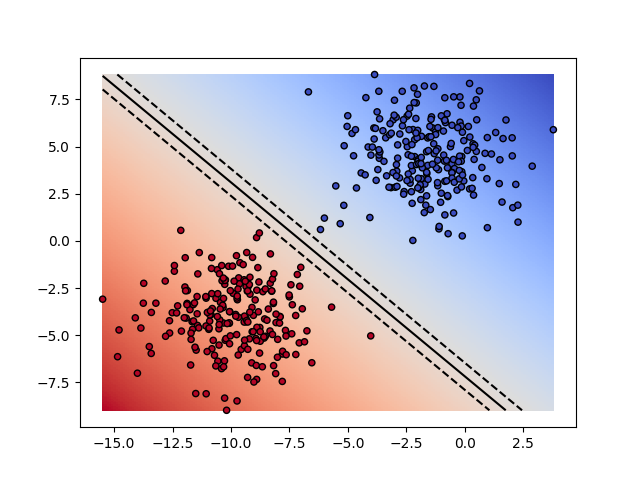
\includegraphics[width=\textwidth]{img/linearsvm.png}
			\end{figure}
	\end{frame}
	
	\begin{frame}
		\frametitle{Einführung: Linear nicht seperierbare Daten 1}
			\begin{figure}
					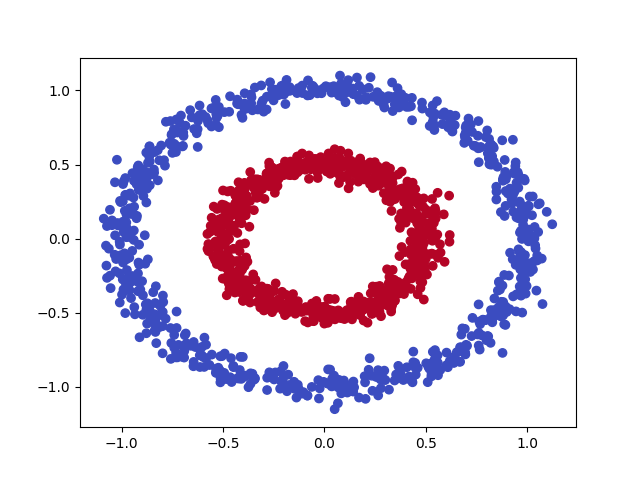
\includegraphics[width=\textwidth]{img/nonlinearsvm.png}
			\end{figure}
	\end{frame}
	
	\begin{frame}
		\frametitle{Einführung: Linear nicht seperierbare Daten 2}
			\begin{figure}
					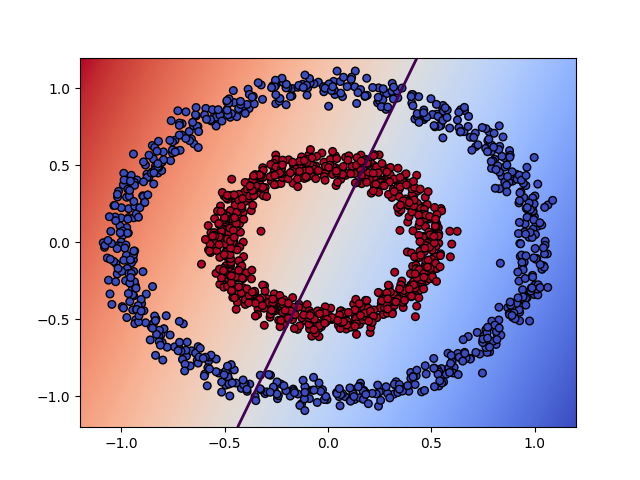
\includegraphics[width=\textwidth]{img/nonlinearsvmwbl.png}
			\end{figure}
	\end{frame}
	
	\begin{frame}
		\frametitle{Ansatz: Einführung}
			\begin{columns}
				\begin{column}{.4\textwidth}
					\begin{figure}
						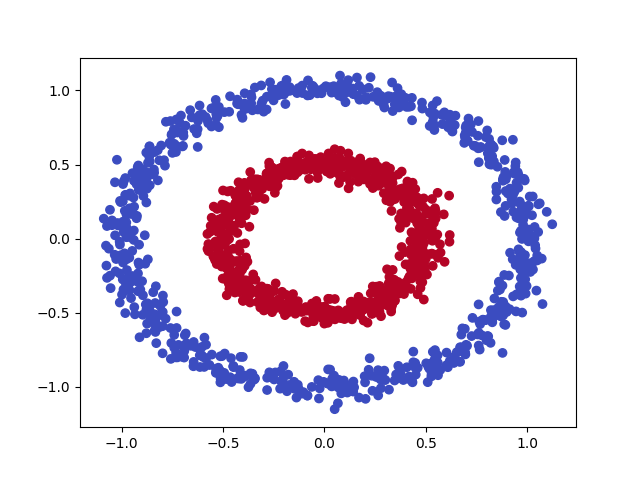
\includegraphics[width=1\textwidth]{img/nonlinearsvm.png}
					\end{figure}
					\begin{align*}
						\phi(\boldsymbol{x}) &=  \begin{bmatrix}
										x_{1} \\
										x_{2} \\
										x_{1}^{\,2} + x_{2}^{\,2}
									\end{bmatrix}
					\end{align*}
				\end{column}
				\begin{column}{.6\textwidth}
				\end{column}
			\end{columns}
	\end{frame}
	\begin{frame}
	\frametitle{Ansatz: Einführung}
		\begin{columns}
			\begin{column}{.4\textwidth}
				\begin{figure}
					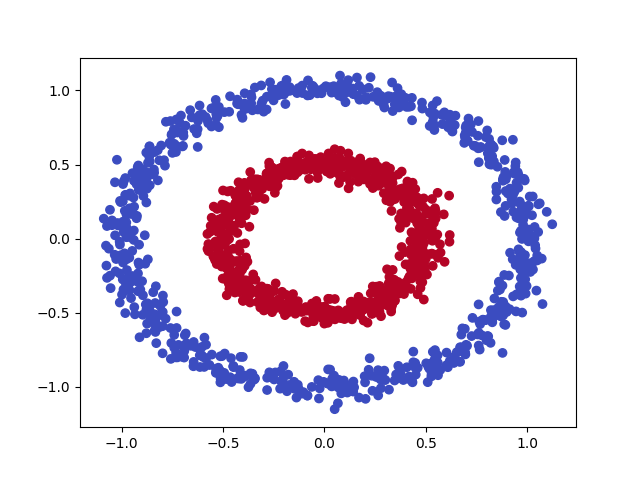
\includegraphics[width=1\textwidth]{img/nonlinearsvm.png}
				\end{figure}
				\begin{align*}
					\phi(\boldsymbol{x}) &=  \begin{bmatrix}
									x_{1} \\
									x_{2} \\
									x_{1}^{\,2} + x_{2}^{\,2}
								\end{bmatrix}
				\end{align*}
			\end{column}
			\begin{column}{.6\textwidth}
				\begin{figure}
					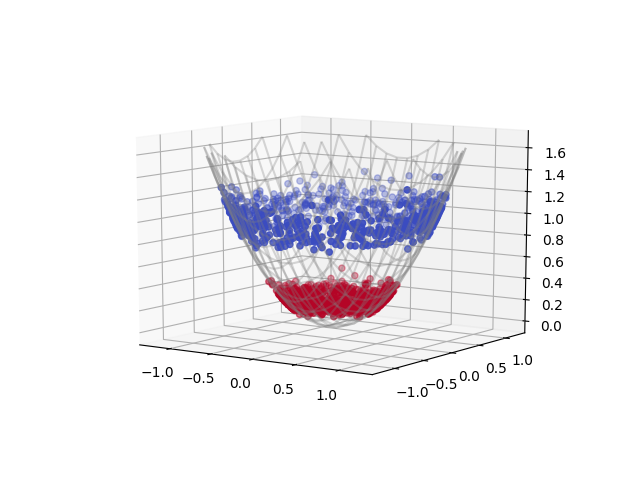
\includegraphics[width=1\textwidth]{img/nonlinearsvm3d.png}
				\end{figure}
				\vspace{45pt}
			\end{column}
		\end{columns}
	\end{frame}
	
	\begin{frame}
		\frametitle{Ansatz: Abbildfunktion $\phi(x)$}
			\begin{columns}
				\begin{column}{.6\textwidth}
					\begin{figure}
							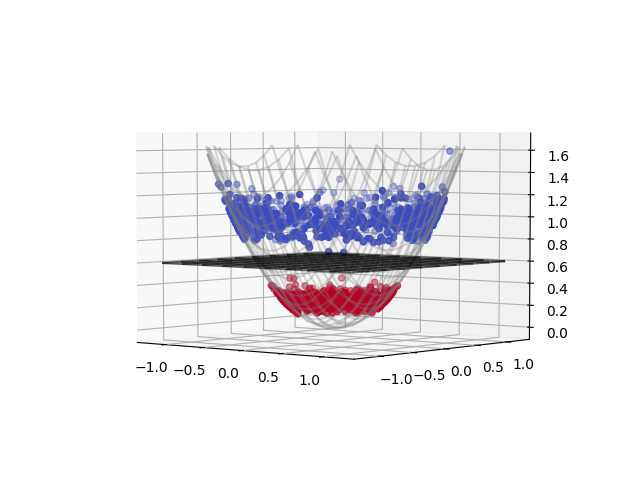
\includegraphics[width=1\textwidth]{img/nonlinearsvm3dwb.png}
					\end{figure}
				\end{column}
				\begin{column}{.4\textwidth}
					\begin{figure}
							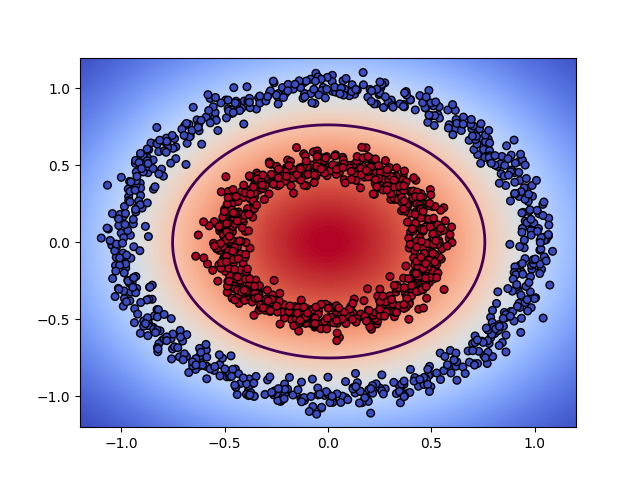
\includegraphics[width=1\textwidth]{img/nonlinearsvmwb.png}
					\end{figure}
				\end{column}
			\end{columns}
	\end{frame}
	
	\begin{frame}
		\frametitle{Veränderung der Funktionen}
			\begin{equation*}
				L = \sum_i \alpha_i - \frac{1}{2} \sum_i \sum_j \alpha_i \alpha_j y_i y_j \boldsymbol{x}_i^{T} \boldsymbol{x}_j
			\end{equation*}
			\onslide<2->{
				\begin{equation*}
					L = \sum_i \alpha_i - \frac{1}{2} \sum_i \sum_j \alpha_i \alpha_j y_i y_j \textcolor{red}{\phi(}\boldsymbol{x}_i\textcolor{red}{)}^{T} \textcolor{red}{\phi(}\boldsymbol{x}_j\textcolor{red}{)}
				\end{equation*}
			}
			\begin{equation*}
				h(\boldsymbol{x}) = \sum_i \alpha_i y_i \boldsymbol{x}_i^{T} \boldsymbol{x} + b
			\end{equation*}
			\onslide<2->{
				\begin{equation*}
					h(\boldsymbol{x}) = \sum_i \alpha_i y_i \textcolor{red}{\phi(}\boldsymbol{x}_i\textcolor{red}{)}^{T} \textcolor{red}{\phi(}\boldsymbol{x}\textcolor{red}{)} + b
				\end{equation*}
			}
	\end{frame}

\section{Mathematik}
	\begin{frame}
		\frametitle{Genauere Klärung von $\phi$}
			Abbildfunktion
			\begin{align*}
				\phi: \mathbb{R}^{n} & \to \mathbb{R}^{m} \\
				\boldsymbol{x} & \mapsto \boldsymbol{f}
			\end{align*}
			\pause
			Probleme:
			\begin{itemize}
				\item $m > n$ höherer Rechenaufwand \\
					Ab einer bestimmten größe kann damit nicht mehr gerechnet werden
				\item Obergrenze für $m$
				\item $\phi$ nur für Skalarprodukt benötigt
			\end{itemize}
	\end{frame}
	
	\begin{frame}
		\frametitle{Beispiel Kernel}
			\begin{equation*}
				\phi(\boldsymbol{x}) = (1 \ \sqrt{2}x_{1} \ \sqrt{2}x_{2} \ \dots \ x_{1}^{2}x_{2}^{2} \ \dots \ \sqrt{2}x_{1}x_{2} \ \sqrt{2}x_{1}x_{3} \ \dots)
			\end{equation*}
			\pause
			\begin{align*}
				\phi(\boldsymbol{v})^{T}\phi(\boldsymbol{w}) &= \sum_{j} 2v_{j}w_{j} + \sum_{j} v_{j}^{2} w_{j}^{2} + \sum_{j} \sum_{k > j} 2 v_{j} v_{k} w_{j} w_{k} + \dots \\
						&= (1+\sum_{j} v_{j} w_{j})^{2} \\
						&= (1+\boldsymbol{v}^{T} \boldsymbol{w})^{2} \\
						&= K(\boldsymbol{v}, \boldsymbol{w})
			\end{align*}
	\end{frame}
	
	\begin{frame}
		\frametitle{Einführung von Kerneln}
			\begin{align*}
				K&(\boldsymbol{v}, \boldsymbol{w}) = \phi(\boldsymbol{v})^{T} \phi(\boldsymbol{w})\\
				K&: \mathbb{R}^n \times \mathbb{R}^n \rightarrow \mathbb{R}
			\end{align*}
			\pause
			\begin{equation*}
				L = \sum_i \alpha_i - \frac{1}{2} \sum_i \sum_j \alpha_i \alpha_j y_i y_j \textcolor{red}{K(}\boldsymbol{x}_i\textcolor{red}{,} \boldsymbol{x}_j\textcolor{red}{)}
			\end{equation*}
			\begin{equation*}
				h(\boldsymbol{x}) = \sum_i \alpha_i y_i \textcolor{red}{K(}\boldsymbol{x}_i\textcolor{red}{,} \boldsymbol{x}\textcolor{red}{)} + b
			\end{equation*}
	\end{frame}
	
	\begin{frame}
		\frametitle{Mercer's Theorem: 1}
			$\{ \boldsymbol{x}^{(1)}, \dots, \boldsymbol{x}^{(m)} \}$ \\
			$\mathcal{K}_{i,j} = K(\boldsymbol{x}^{(i)}, \boldsymbol{x}^{(j)})$ \\\
			\pause
			
			\begin{align*}
				\mathcal{K}_{i,j} &= K(\boldsymbol{x}^{(i)}, \boldsymbol{x}^{(j)}) \\
								  &= \phi(\boldsymbol{x}^{(i)})^{T} \phi(\boldsymbol{x}^{(j)}) \\
								  &= \phi(\boldsymbol{x}^{(j)})^{T} \phi(\boldsymbol{x}^{(i)}) \\
								  &= K(\boldsymbol{x}^{(j)}, \boldsymbol{x}^{(i)}) \\
								  &= \mathcal{K}_{j,i}
			\end{align*}
	\end{frame}
	
	\begin{frame}
		\frametitle{Mercer's Theorem: 2}
			$\{ \boldsymbol{x}^{(1)}, \dots, \boldsymbol{x}^{(m)} \}$ \\
			$\mathcal{K}_{i,j} = K(\boldsymbol{x}^{(i)}, \boldsymbol{x}^{(j)})$ \\\
			
			Wähle $\boldsymbol{z}$ beliebig:
			\begin{align*}
				\boldsymbol{z}^{T} \mathcal{K} \boldsymbol{z} &= \sum_{i} \sum_{j} \boldsymbol{z}_{i} \mathcal{K}_{i,j} \boldsymbol{z}_{j} \\
															  &= \sum_{i} \sum_{j} \boldsymbol{z}_{i} \phi(\boldsymbol{x}^{(i)})^{T} \phi(\boldsymbol{x}^{(j)}) \boldsymbol{z}_{j} \\
															  &= \sum_{i} \sum_{j} \boldsymbol{z}_{i} \sum_{k} \phi_{k}(\boldsymbol{x}^{(i)})^{T} \phi_{k}(\boldsymbol{x}^{(j)}) \boldsymbol{z}_{j} \\
															  &= \sum_{k} \sum_{i} \sum_{j} \boldsymbol{z}_{i} \phi_{k}(\boldsymbol{x}^{(i)})^{T} \phi_{k}(\boldsymbol{x}^{(j)}) \boldsymbol{z}_{j} \\
															  &= \sum_{k} \left( \sum_{i} \boldsymbol{z}_{i} \phi_{k}(\boldsymbol{x}^{(i)}) \right)^{2} \\
															  &\ge 0 \\
			\end{align*}
	\end{frame}
	
	% \begin{frame}
	% 	\frametitle{Kernel Operationen: Addition}
	% 		Addition \\
	% 		\begin{align*}
	% 			(K_{1} + K_{2})(\boldsymbol{v}, \boldsymbol{w}) &= K_{1}(\boldsymbol{v}, \boldsymbol{w}) + K_{2}(\boldsymbol{v}, \boldsymbol{w}) \\
	% 			&= \phi_{1}(\boldsymbol{v})^{T}\phi_{1}(\boldsymbol{w}) + \phi_{2}(\boldsymbol{v})^{T}\phi_{2}(\boldsymbol{w}) \\
	% 			&= (\phi_{1}(\boldsymbol{v}), \phi_{2}(\boldsymbol{v})) \left( \begin{matrix}
	% 													  	\phi_{1}(\boldsymbol{w}) \\
	% 													  	\phi_{2}(\boldsymbol{w})
	% 													  \end{matrix} \right)
	% 		\end{align*}
	% \end{frame}
	% \begin{frame}
	% 	\frametitle{Kernel Operationen: Multiplikation}
	% 		Multiplikation \\
	% 		\begin{align*}
	% 			(K_{1} \times K_{2})(\boldsymbol{v}, \boldsymbol{w}) &= K_{1}(\boldsymbol{v}, \boldsymbol{w}) K_{2}(\boldsymbol{v}, \boldsymbol{w}) \\
	% 			&= \sum_{i=1}^{n} \phi_{1i}(\boldsymbol{v})\phi_{1i}(\boldsymbol{w}) \sum_{j=1}^{m} \phi_{2j}(\boldsymbol{v})\phi_{2j}(\boldsymbol{w}) \\
	% 			&= \sum_{i=1}^{n} \sum_{j=1}^{m} (\phi_{1i}(\boldsymbol{v})\phi_{2j}(\boldsymbol{v}))(\phi_{1i}(\boldsymbol{w})\phi_{2j}(\boldsymbol{w})) \\
	% 			&= \sum_{k=1}^{nm} \phi_{12k}(\boldsymbol{v})\phi_{12k}(\boldsymbol{w}) = \phi_{12}(\boldsymbol{v})^{T}\phi_{12k}(\boldsymbol{w})
	% 		\end{align*}
	% 		Mit $\phi_{12}(\boldsymbol{x}) = \phi_{1}(\boldsymbol{x}) \times \phi_{2}(\boldsymbol{x})$ dem kartesischen Produkt
	% \end{frame}
	
	\begin{frame}
		\frametitle{Verschiedene Kernel in der Praxis}
			\begin{itemize}
				\item Linearer Kernel \\
				\item Gauß'schen Kernel \\
				\item Polynomiell \\
				\item Esotherische Kernel \\
			\end{itemize}
	\end{frame}

	\begin{frame}
		\frametitle{Verschiedene Kernel in der Praxis: Linear}
			\vspace{10pt}
			$K(\boldsymbol{v}, \boldsymbol{w}) = \boldsymbol{v}^{\, T} \boldsymbol{w}$
			\begin{figure}
				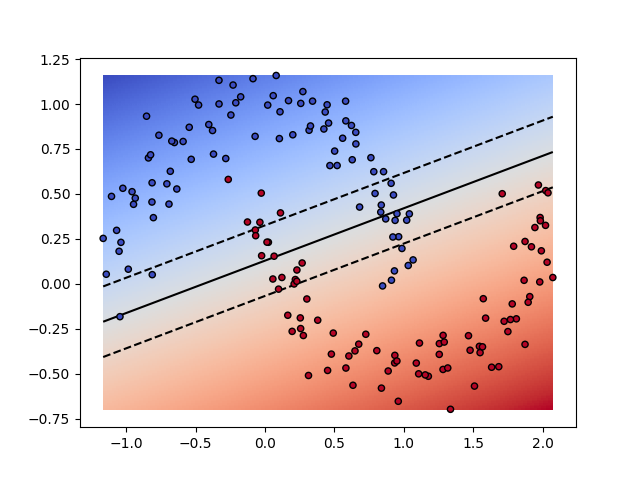
\includegraphics[width=.9\textwidth]{img/kernelLin.png}
			\end{figure}
	\end{frame}
	
	\begin{frame}
		\frametitle{Verschiedene Kernel in der Praxis: Polynomiell}
			\vspace{10pt}
			$K(\boldsymbol{v}, \boldsymbol{w}) = (\boldsymbol{v}^{\, T} \boldsymbol{w} + c)^{d}$
			\begin{figure}
				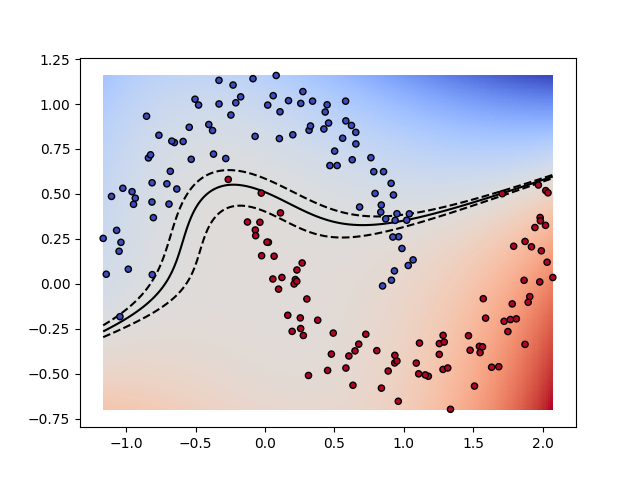
\includegraphics[width=.9\textwidth]{img/kernelPol.png}
			\end{figure}
	\end{frame}
	
	\begin{frame}
		\frametitle{Verschiedene Kernel in der Praxis: Gauß}
			\vspace{10pt}
			$K(\boldsymbol{v}, \boldsymbol{w}) = \exp(-\frac{\lvert\lvert\boldsymbol{v} - \boldsymbol{w}\rvert\rvert^{2}}{2\sigma^{2}})$ \\\
			
			\begin{columns}
				\begin{column}{.5\textwidth}
					\begin{figure}
						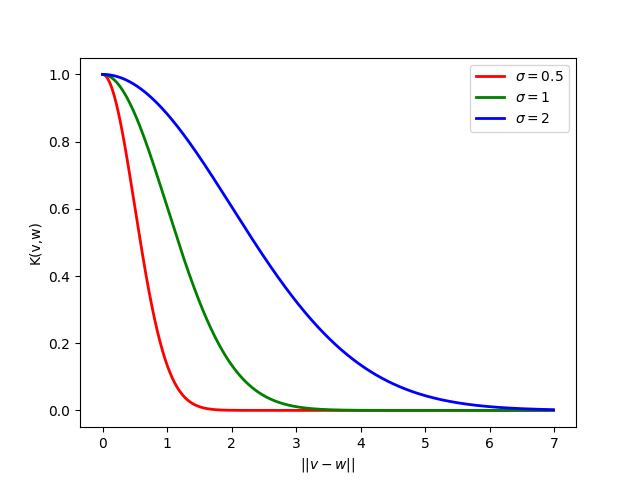
\includegraphics[width=\textwidth]{img/sigmaGau.png}
					\end{figure}
				\end{column}
				\begin{column}{.5\textwidth}
					\begin{figure}
						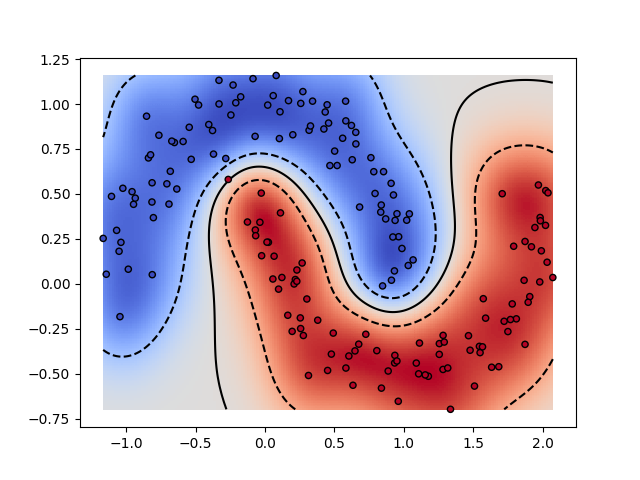
\includegraphics[width=\textwidth]{img/kernelGau.png}
					\end{figure}
				\end{column}
			\end{columns}
	\end{frame}
	
	\begin{frame}
		\frametitle{Verschiedene Kernel in der Praxis: "Esotherisch"}
			$K: D \times D \rightarrow \mathbb{R}$ \\\
			
			Beispiel: String Kernel \\
			\hspace{31pt} Misst Ähnlichkeit von zwei Strings \\
			\hspace{31pt} Vergleicht verschiedene Aspekte \\
			\hspace{62pt} e.g. Subequenzen, gemeinsame Wörter, Länge, $\dots$
	\end{frame}
	
\section{Zusammenfassung}
	\begin{frame}
		\frametitle{Zusammenfassung}
			\begin{itemize}
				\item SVMs in ihrer Standartform haben Probleme nicht liear trennbare Datensätze zu klassifizieren
				\item Mit $\phi(x)$ Daten in einen Raum abbilden wo dies möglich ist
				\item Kernel nutzen um die daraus folgende Berechnung zu vereinfachen
			\end{itemize}
	\end{frame}

% \section{Quellen}
	% \begin{frame}
	% 	\frametitle{Quellen}
	% 		{\footnotesize \printbibliography[title={Whole bibliography}]}
	% Kernelmath: http://disi.unitn.it/~passerini/teaching/2013-2014/MachineLearning/slides/17_kernel_machines/handouts.pdf
	% \end{frame}
